\documentclass[12pt,a4paper]{article}
\usepackage[margin=1in]{geometry}
\usepackage{amsmath}
\usepackage{graphicx}
\usepackage{booktabs}
\usepackage{caption}
\usepackage{parskip}
\usepackage{float}

\title{\textbf{E0-270o: Machine Learning: Assignment 3}\\[0.5em]
       \large Support Vector Machines and CNN on FashionMNIST}
\author{Dinesh Chand}
\date{April 2026}

\begin{document}
\maketitle

\section{Task 1: Multi-Class SVM}

\subsection{Methodology}

FashionMNIST images are $28 \times 28$ grayscale, so each image is a 784-dimensional
vector when flattened. PCA is applied before SVM training to reduce this
dimensionality — both to speed up training and to remove noise from less important
directions. PCA is fit on the training set only, and the same projection is then
applied to the test set.

The 1-vs-Rest strategy is used: one binary SVM is trained per class (10 total), and
the predicted class is whichever SVM returns the highest decision score $w^Tx + b$.

\subsubsection{SVM Formulation}

The soft-margin SVM minimizes the following objective:
\[
\min_{w,\, b} \;\; \|w\|_2^2 \;+\; C \sum_{n=1}^{N} \max\!\bigl(0,\; 1 - y_n(w^T x_n + b)\bigr)
\]
This unconstrained problem is solved using SGD. At each step one training sample
$(x_i, y_i)$ is drawn at random and the update uses the subgradient:
\[
\nabla_w =
\begin{cases}
2w & \text{if } y_i(w^Tx_i + b) \geq 1 \\
2w - C \cdot y_i \cdot x_i & \text{otherwise}
\end{cases}
\qquad
\nabla_b =
\begin{cases}
0 & \text{if } y_i(w^Tx_i + b) \geq 1 \\
-C \cdot y_i & \text{otherwise}
\end{cases}
\]
At the boundary ($y_i(w^Tx_i + b) = 1$) the subgradient is taken as zero, which is
a valid subgradient of the hinge loss at that point.

\subsubsection{Learning Rate Schedule}

A linear decay schedule is used: $\eta_t = \eta_0\,/\,(1 + t/T)$, where $\eta_0 = 10^{-3}$
and $T$ is the total number of iterations. Under this schedule the learning rate only
halves by the final step, so all iterations contribute meaningfully to training.
A $1/\sqrt{t}$ schedule was also tried but it decayed too aggressively — by step 10,000
the effective step size had shrunk to around $10^{-5}$, and the model barely updated
in the later half of training. The comparison in Figure~\ref{fig:lr_compare} (see Results)
shows the linear schedule consistently outperforms $1/\sqrt{t}$ decay across all $k$.

\subsection{Hyperparameters}

\begin{itemize}
    \item Regularisation constant: $C = 1.0$
    \item Initial learning rate: $\eta_0 = 10^{-3}$
    \item SGD iterations per binary SVM: 10,000
    \item PCA components tested: $k \in \{10, 20, 50, 100, 200, 300, 400\}$
\end{itemize}

\subsection{Results}

Table~\ref{tab:svm} shows the test set performance for each value of $k$.
All metrics are macro-averaged across the 10 classes, which is appropriate since
FashionMNIST is a balanced dataset (1,000 test samples per class).

\begin{table}[h]
\centering
\caption{Test set metrics vs number of PCA components ($C = 1.0$)}
\label{tab:svm}
\begin{tabular}{@{}ccccc@{}}
\toprule
$k$ & Accuracy & Precision & Recall & F1 \\
\midrule
10  & 0.6365 & 0.6041 & 0.6365 & 0.5833 \\
20  & 0.6542 & 0.6915 & 0.6542 & 0.6105 \\
50  & 0.7162 & 0.7136 & 0.7162 & 0.7068 \\
100 & 0.7269 & 0.7456 & 0.7269 & 0.6989 \\
200 & 0.7355 & 0.7622 & 0.7355 & 0.7108 \\
300 & 0.7419 & 0.7458 & 0.7419 & 0.7230 \\
400 & 0.7606 & 0.7652 & 0.7606 & 0.7439 \\
\bottomrule
\end{tabular}
\end{table}

\begin{figure}[H]
\centering
\begin{minipage}{0.48\textwidth}
    \centering
    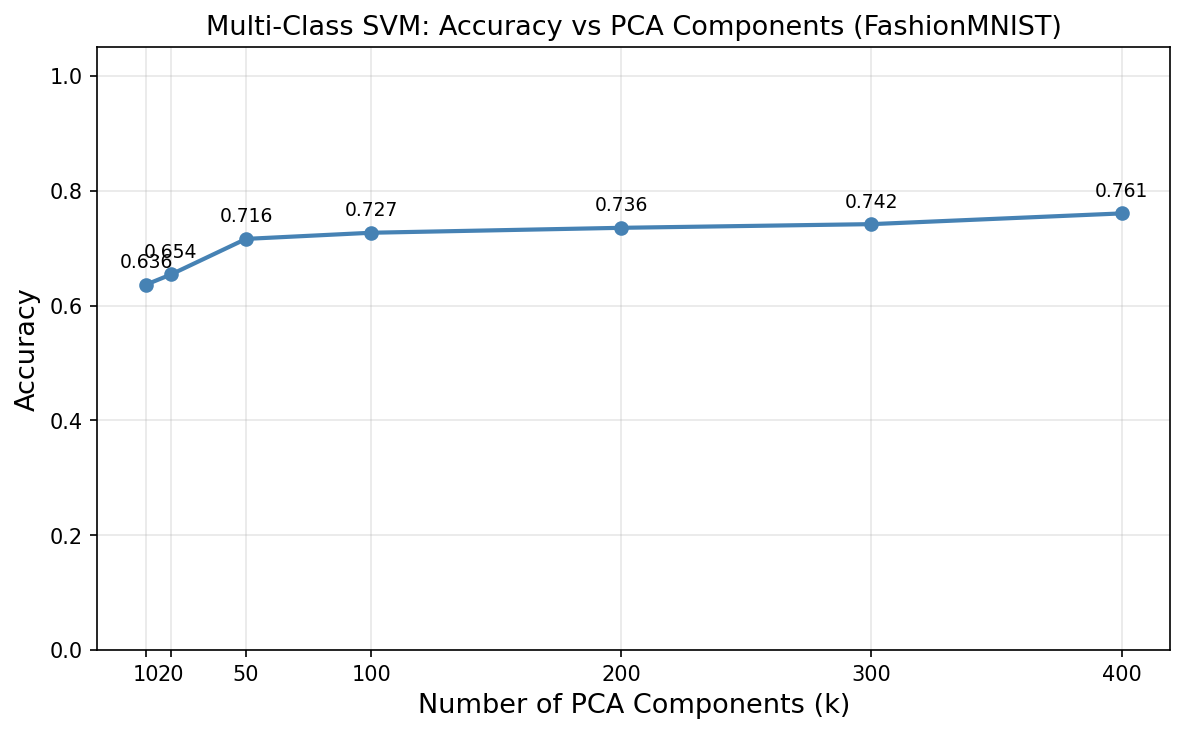
\includegraphics[width=\textwidth]{plots/svm_accuracy_vs_pca_components.png}
    \caption{Accuracy vs PCA components.}
    \label{fig:svm_acc}
\end{minipage}
\hfill
\begin{minipage}{0.48\textwidth}
    \centering
    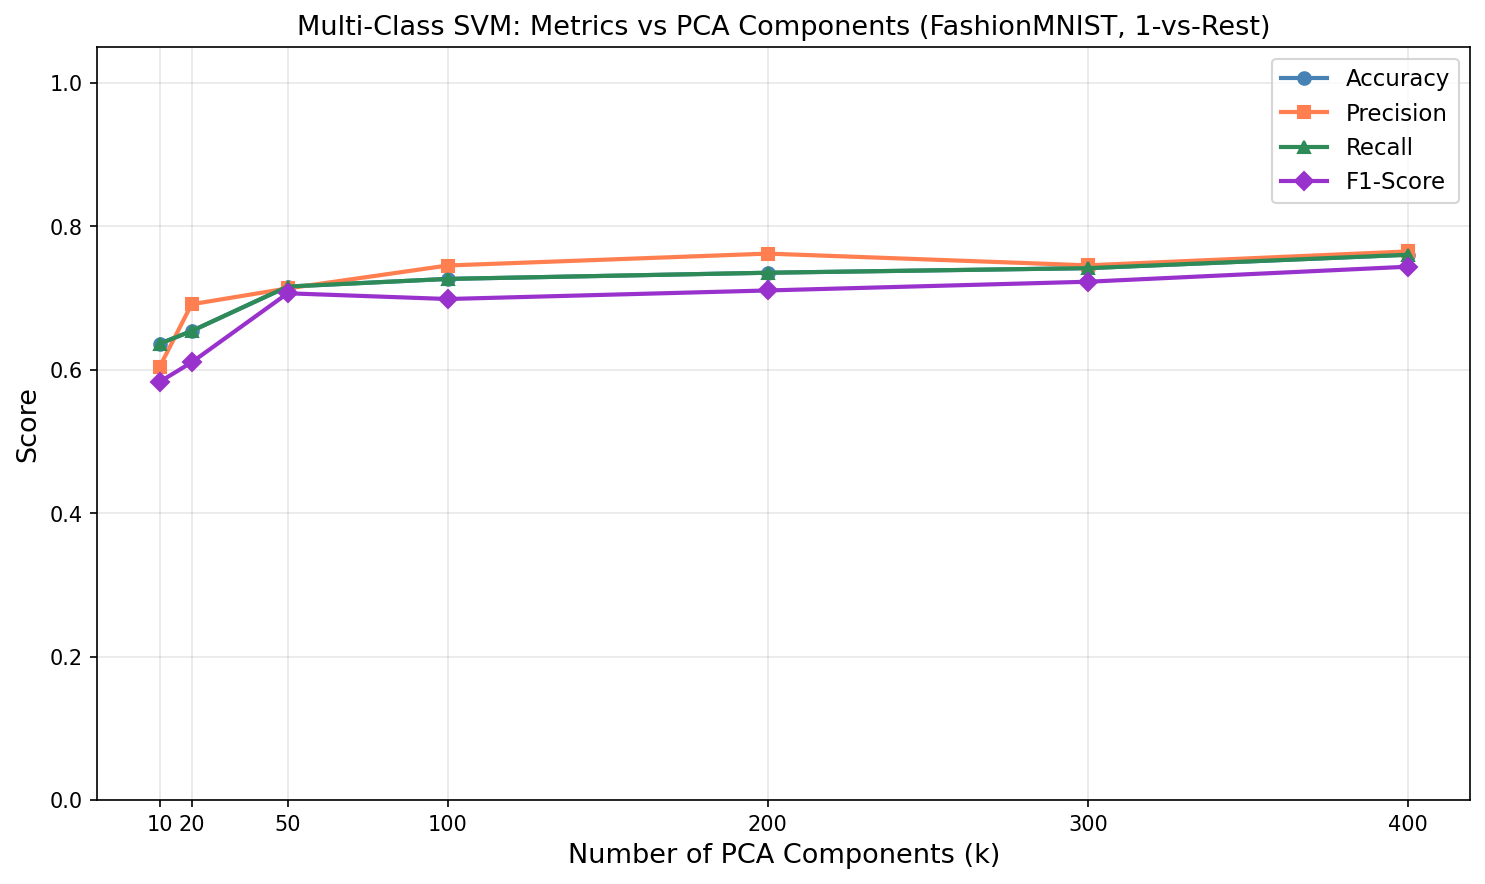
\includegraphics[width=\textwidth]{plots/svm_metrics_vs_pca_components.png}
    \caption{All metrics vs PCA components.}
    \label{fig:svm}
\end{minipage}
\end{figure}

\begin{figure}[H]
\centering
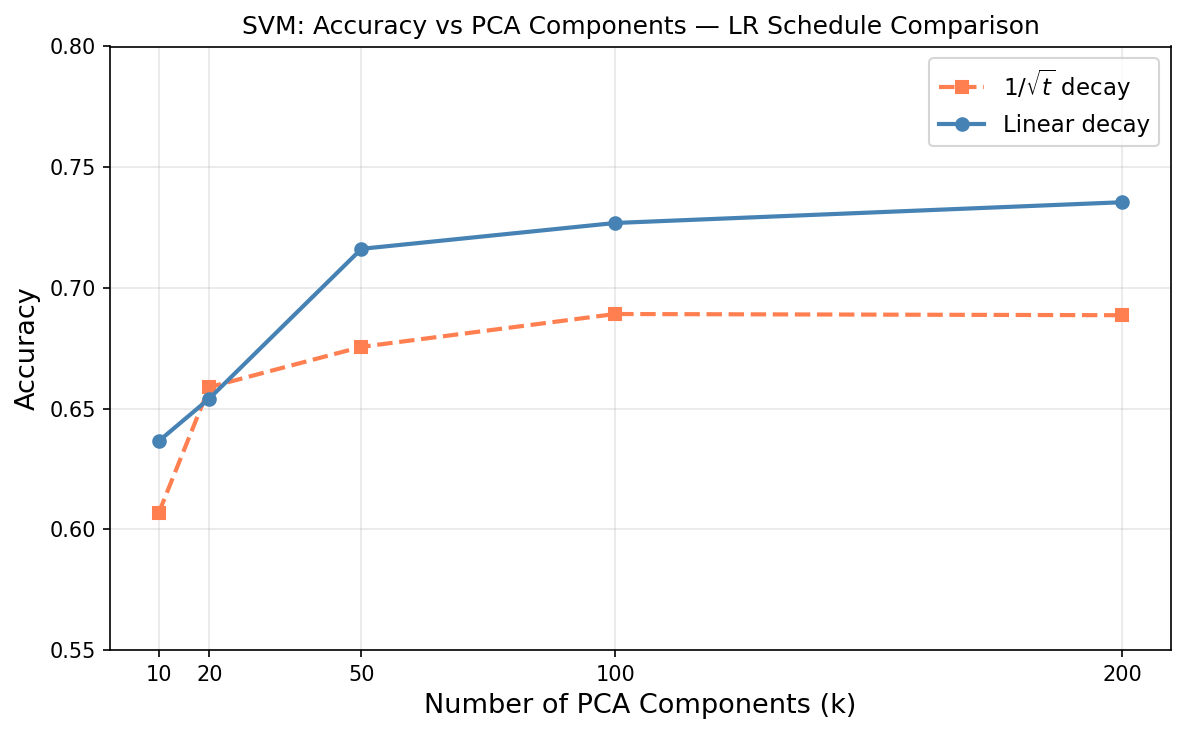
\includegraphics[width=0.75\textwidth]{plots/svm_lr_schedule_comparison.png}
\caption{Accuracy vs PCA components for the two learning rate schedules.
         Linear decay consistently outperforms $1/\sqrt{t}$ decay across all $k$.}
\label{fig:lr_compare}
\end{figure}

\subsection{Analysis}

The most notable observation in Figures~\ref{fig:svm_acc} and~\ref{fig:svm} is the jump between $k=20$ and
$k=50$, where accuracy goes from 65.4\% to 71.6\% (+6.2\%). The first 50 principal
components capture the bulk of the discriminative structure in the images (overall
shape, contrast patterns), while the components beyond that describe finer details.
The gains continue but at a slower pace all the way to $k=400$.

The trend is strictly monotone throughout, so even at 400 components the model
continues to benefit from the additional directions. Going much beyond 400 would
start to defeat the purpose of PCA, since the remaining components would capture
noise rather than useful signal.

Precision is slightly higher than recall at larger $k$, meaning the model tends to
be conservative — it predicts a class only when fairly confident, which keeps false
positives low but misses some true positives. The gap between precision and recall
is small though, and all four metrics follow a similar trend overall.

The model reaches around 76\% accuracy at $k=400$, which is a reasonable
result for a linear SVM with no feature engineering beyond PCA.

\section{Task 2: Convolutional Neural Network}

\subsection{Methodology}

A convolutional neural network is trained directly on the FashionMNIST images
without any dimensionality reduction. Each image is kept in its original
$28 \times 28$ format and fed to the network as a single-channel tensor.
The pixel values are normalized using the training set mean ($\mu = 0.2860$)
and standard deviation ($\sigma = 0.3530$).

\subsubsection{Architecture}

The network follows a LeNet-style design with two convolutional blocks followed
by fully connected layers.

\begin{itemize}
    \item \textbf{Block 1:} Conv2d($1 \to 6$, kernel $5\times5$) $\to$ BatchNorm $\to$ ReLU $\to$ MaxPool2d($2\times2$) \\
          Output: $6 \times 12 \times 12$
    \item \textbf{Block 2:} Conv2d($6 \to 16$, kernel $5\times5$) $\to$ BatchNorm $\to$ ReLU $\to$ MaxPool2d($2\times2$) \\
          Output: $16 \times 4 \times 4$
    \item \textbf{FC layers:} $256 \to 120 \to 84 \to 10$
\end{itemize}

BatchNorm is added after each convolution to stabilise training. The output
layer produces 10 logits (one per class), and the predicted class is the
argmax of these logits.

\subsubsection{Training}

The network is trained using Cross-Entropy loss and the Adam optimizer
($\text{lr} = 10^{-3}$) for 20 epochs with a batch size of 64.
After each epoch the model is evaluated on the test set and all four
metrics are recorded.

\subsection{Hyperparameters}

\begin{itemize}
    \item Optimizer: Adam, learning rate $10^{-3}$
    \item Loss: Cross-Entropy
    \item Batch size: 64
    \item Epochs: 20
\end{itemize}

\subsection{Results}

Table~\ref{tab:cnn} shows the final test set metrics after 20 epochs of training.
All metrics are macro-averaged across the 10 classes.

\begin{table}[h]
\centering
\caption{CNN final test set metrics (epoch 20)}
\label{tab:cnn}
\begin{tabular}{@{}lr@{}}
\toprule
Metric    & Score  \\
\midrule
Accuracy  & 0.8910 \\
Precision & 0.8927 \\
Recall    & 0.8910 \\
F1        & 0.8896 \\
\bottomrule
\end{tabular}
\end{table}

\begin{figure}[H]
\centering
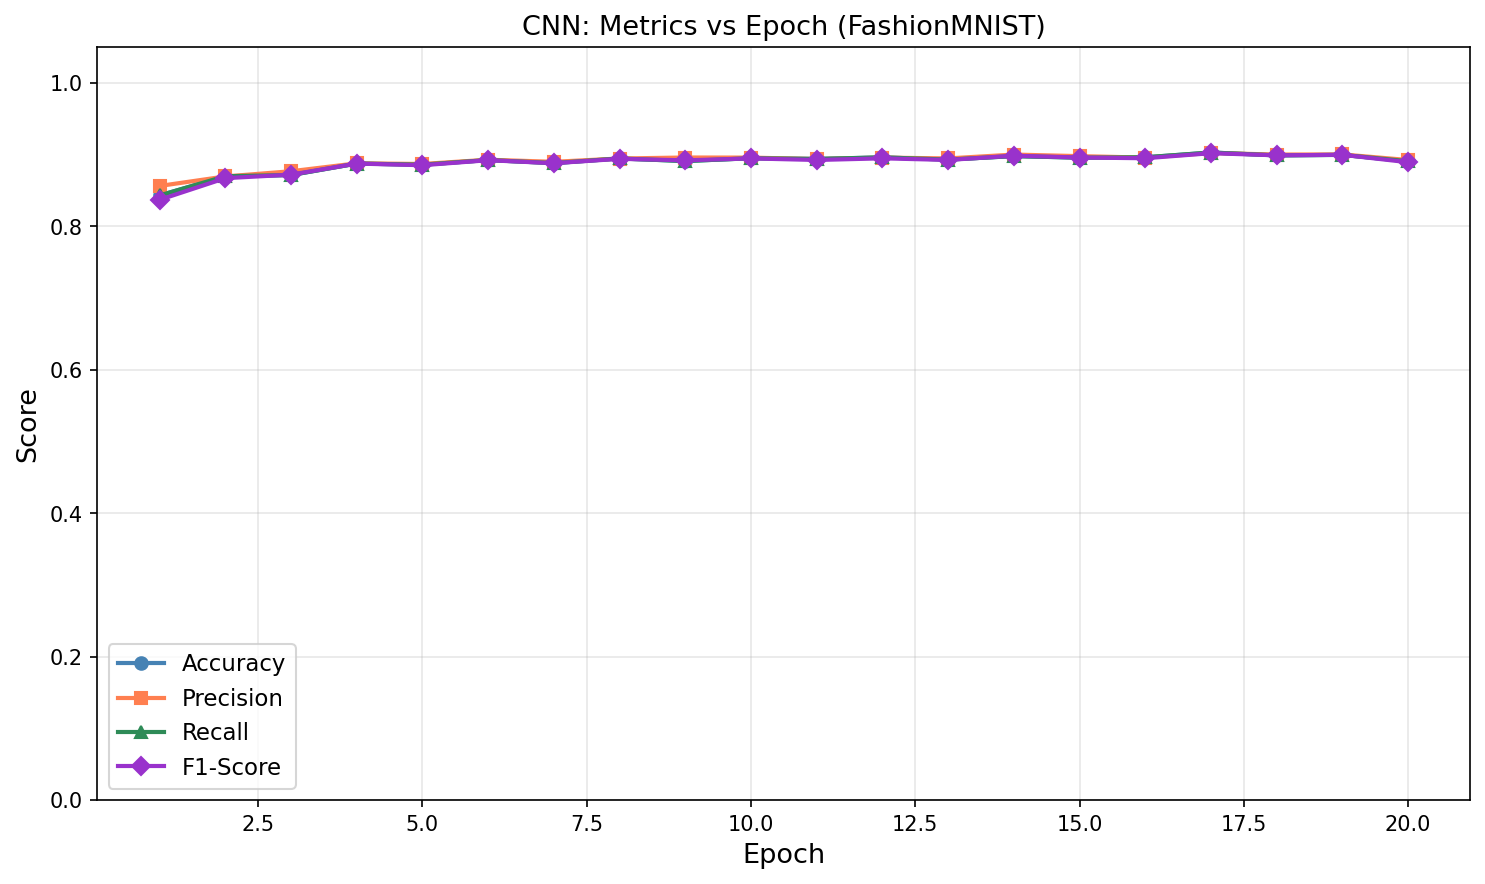
\includegraphics[width=0.85\textwidth]{plots/cnn_metrics_vs_epoch.png}
\caption{Accuracy, Precision, Recall, and F1 vs epoch for the CNN on FashionMNIST.}
\label{fig:cnn}
\end{figure}

\subsection{Analysis}

Figure~\ref{fig:cnn} shows how the metrics evolve over training. Most of the
improvement happens in the first 6 epochs (84.3\% $\to$ 89.3\%), after which
the test accuracy oscillates around 89–90\% with no clear upward trend. The
training loss continues to decrease throughout, while test accuracy has plateaued
— a sign of mild overfitting in the later epochs. The best single-epoch result
was epoch 17 (90.3\%).

The CNN reaches 89.1\% accuracy at epoch 20, compared to 76.1\% for the best
SVM configuration ($k=400$). The gap of around 13\% reflects the advantage of
convolutional layers, which can capture local spatial structure (edges, textures,
shapes) that a linear classifier operating on PCA features cannot.

Precision and recall stay very close throughout training, consistent with the
balanced class distribution in FashionMNIST.

\end{document}
